\documentclass[11pt]{article}
\usepackage{geometry, titlesec}
\usepackage[parfill]{parskip}
\usepackage[italicdiff]{physics}
\usepackage{amsfonts, amsthm}
\usepackage[cm]{fullpage}
\usepackage{fancyhdr}
\usepackage{enumitem}
\usepackage{xcolor, soul}
\usepackage{graphicx}
\usepackage[export]{adjustbox}
\usepackage{siunitx}
%\allowdisplaybreaks

\renewcommand{\thesubsection}{\thesection.\alph{subsection}}
\setenumerate[1]{label={(\alph*)}}

\makeatletter
\renewcommand*\env@cases[1][1.2]{%
  \let\@ifnextchar\new@ifnextchar
  \left\lbrace
  \def\arraystretch{#1}%
  \array{@{}l@{\quad}l@{}}%
}
\makeatother
 
\renewcommand{\footrulewidth}{.2pt}
%\setlist[enumerate]{leftmargin=*}
\pagestyle{fancy}
\fancyhf{}
\lhead{Physics 132-B}
\chead{\textbf{Discussion 7 Problems}}
\rhead{A--De Discussion}
\setlength{\headheight}{11pt}
\setlength{\headsep}{11pt}
\setlength{\footskip}{24pt}
\lfoot{\today}
\rfoot{\thepage}

\titleformat{\subsection}[runin]{\normalfont\large\bfseries}{\thesubsection}{1em}{}
\newcommand{\refeq}[1]{(\ref{#1})}

\newcommand{\beq}{\begin{equation*}}
\newcommand{\eeq}{\end{equation*}}

\newcommand{\beqn}{\begin{equation}}
\newcommand{\eeqn}{\end{equation}}

\newcommand{\blg}{\begin{align*}}
\newcommand{\elg}{\end{align*}}


\newenvironment{statement}
{
%    \color{gray}
    \ignorespaces
}
{
%    \smallskip
}

\newenvironment{problem}
{
    \color{darkgray}
    \ignorespaces
}

\newenvironment{solution}
{
    \paragraph{Solution.}
    \ignorespaces
}
{
    \bigskip
}

\newcommand{\qimplies}{\quad \implies \quad}


\begin{document}
	


\newcommand{\vF}{\vb{F}}
\newcommand{\vv}{\vb{v}}
\newcommand{\vB}{\vb{B}}

\paragraph{Question 27.1}
\begin{problem}
	Can a charged particle move through a magnetic field without experiencing any force?  If so, how?  If not, why not?
\end{problem}

\begin{solution}
	The magnetic force on a particle of charge $q$ is given by $\vF = q \vv \times \vB$, where $\vv$ is the particle's velocity and $\vB$ is the magnetic field.  The cross product $\vv \times \vB$ is zero if $\vv$ and $\vB$ are parallel.  In this case, $\vF = 0$.  So yes, a charged particle can move through a magnetic field without experiencing any force, as long as it is moving parallel to the field.
\end{solution}

\vfill

\paragraph{Question 27.7}
\begin{problem}
	If the magnetic force does no work on a charged particle, how can it have any effect on the particle's motion?  Are there other examples of forces that do no work but have a significant effect on a particle's motion?
\end{problem}

\begin{solution}
	It is certainly possible for a force to affect motion without doing work.  Think back to the mechanics problems we studied last quarter, and imagine a hockey puck sliding horizontally on some (frictionless) ice.  If someone blocks the puck with a hockey stick, they are exerting a force on the puck, which will bounce off.  The puck's direction of motion will change depending on the position of the hockey stick.  However, the velocity of the puck remains the same~(assuming a perfectly elastic collision), so the energy of the puck hasn't changed, and therefore no work has been done.  The magnetic force similarly is able to change the direction of a particle without doing work.
\end{solution}

\vfill

\paragraph{Question 28.4}
\begin{problem}
	Two parallel conductors carrying current in the same direction attract each other.  If they are permitted to move toward each other, the forces of attraction do work.  From where does the energy come?  Does this contradict the assertion in Chapter 27 that magnetic forces on moving charges do no work?  Explain.
\end{problem}

\begin{solution}
	Magnetic forces are not the only thing we have to think about for this system.  The conductors are carrying current, so they must be connected to a power source.  The power source creates a potential difference which causes a current to flow.  The energy to move the conductors therefore comes from the power source.  This does not contradict the assumption that magnetic forces do no work.  The power source does the work; the magnetic field just delivers the force to the conductors.
\end{solution}

\vfill
%\clearpage

\paragraph{Question 28.10}
\begin{problem}
	What are the relative advantages and disadvantages of Ampere's law and the law of Biot and Savart for practical calculations of magnetic fields?
\end{problem}

\begin{solution}
	This is like comparing Coulomb's law and Gauss's law.  Coulomb's law can tell us the electric field for \emph{any} charge distribution, but actually executing it usually involves calculus and can be difficult.  On the other hand, Gauss's law can only be used when we have certain symmetries, but it makes calculating the electric field in these cases very easy.
	
	Likewise, the Biot-Savart law can be used to calculate the magnetic field for \emph{any} current distribution, but it involes calculus and cross products.  Ampere's law can only be used for certain symmetric configurations, but it is mathematically much easier to implement when it is an option.
\end{solution}

\clearpage


\newcommand{\tht}{\theta}
\newcommand{\muo}{\mu_0}
\newcommand{\lam}{\lambda}
\newcommand{\vL}{\vb{L}}

\begin{minipage}[l]{0.65\textwidth}
\paragraph{Problem 28.61}
\begin{problem}
	Two long, parallel wires hang by a \SI{4.00}{\cm}-long cords from a common axis~(\textbf{Fig.~P28.61}).  The wires have a mass per unit length of \SI{0.0125}{\kg\per\meter} and carry the same current in opposite directions.  What is the current in each wire if the cords hang at an angle of \SI{6.00}{\degree} with the vertical?
\end{problem}
\end{minipage}%
\hspace{0.05\textwidth}%
\begin{minipage}{0.30\textwidth}
\center 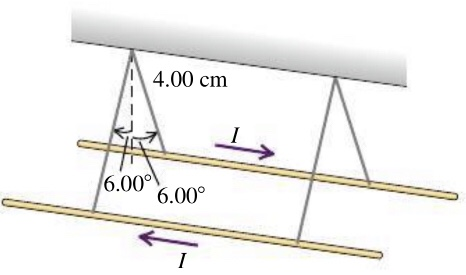
\includegraphics[width=\textwidth]{P28-61.jpeg}
\center \textbf{Figure P28.61}
\end{minipage}

\begin{solution}
	We need to use force balance to find the force that the wires exert on each other, and from that we can find the current.  We can do this by examining just one of the wires.  Let $m g$ be the force of gravity on one wire, $T$ the tension force of the cord holding it up, $\tht$ its angle from the horizontal, and $F$ the electromagnetic force exerted by the other wire.  The force diagram looks something like this:
	
	\begin{center} 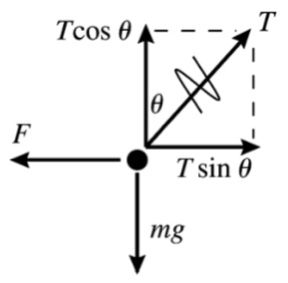
\includegraphics[scale=.4]{P28-61a.jpeg} \end{center}
	
	Balancing forces in the $y$ direction, we find
	\beq
		T \cos\tht = mg
		\qimplies
		T = \frac{m g}{\cos\tht}.
	\eeq
	Balancing forces in the $x$ direction and plugging in $T$ gives us
	\beq
		F = T \sin\tht = \frac{mg}{\cos\tht} \sin\tht = mg \tan\tht.
	\eeq
	The mass $m$ of one of the wires is $\lam L$, where $\lam$ is its mass per unit length and $L$ its total length.  So we have
	\beq
		F = \lam L g \tan\tht
	\eeq
	as the electromagnetic force exerted by the other wire.
	
	Now we need the form of $F$ in terms of the current $I$.  Recall (from Ex.~28.7 in the textbook) that the magnetic field set up by a line of current is
	\beq
		B = \frac{\muo}{2\pi} \frac{I}{r}
	\eeq
	and that the force exerted on the other wire can be found by
	\beq
		\vF = I \vL \times \vB,
	\eeq
	where $I$ is the current flowing through the second wire and $\vL$ is a vector pointing in the direction of the current with magnitude equal to the wire's length $L$.  The magnitude of the force exerted by one wire on the other is
	\beq
		F = \frac{\muo}{2\pi} \frac{I^2 L}{r},
	\eeq
	where $I$ is the current flowing through the wire, $L$ is its length, and $r$ is the distance between the two wires.  Using trigonometry, the distance between the two wires is
	\beq
		r = 2 l \sin\tht,
	\eeq
	where $l$ is the length of each cord.
	
	Equating our two expressions for $F$, we can solve for $I$:
	\beq
		\frac{\muo I^2}{4\pi l \sin\tht} L = \lam L g \tan\tht
		\qimplies
		I^2 = \frac{4\pi}{\muo} \lam l g \sin\tht \tan\tht
		\qimplies
		I = \sqrt{\frac{4\pi}{\muo} \lam l g \sin\tht \tan\tht}.
	\eeq
	Plugging in our given values,
	\beq
		I = \sqrt{\frac{4\pi}{\SI{2e-7}{\tesla\meter\per\ampere}} (\SI{0.0125}{\kg\per\meter}) (\SI{0.0400}{\meter}) (\SI{9.81}{\meter\per\square\second}) \sin(\SI{6.00}{\degree}) \tan(\SI{6.00}{\degree})}
		= {\color{blue} \SI{23.2}{\ampere}}.
	\eeq
	
	
\end{solution}

\vfill 

\end{document}